In this section, the implementation details of the DSU process is described. A proposed format for the \textit{diff} file is presented, as well as the update procedure itself. 
\section{Diff file}\label{sec:patchfile}
To meet the requirements of timeliness and memory usage, an efficient way of describing the update is essential. The method chosen for this project is to use a patch file that describes the changes to be made to the binary image.
The patch file must be minimal in size to keep the transfer- and decode times within the expected idle time. This naturally excludes simply transferring the entire binary image as an option. Instead, a \textit{\textit{diff}}-file is generated by a server system by comparing the current binary to the patched one. For sufficiently small updates, the \textit{diff} file could be as simple as stating addresses to changed instructions and/or data, and the new values for said addresses. This is however not ideal in the case of bigger updates since changes could cause portions of the binary to be shifted, which can be expressed with a \textbf{Shift} operation instead of individual byte- or word-level changes. Consider the example in listings [\ref{lst:shift_example_pre}, \ref{lst:shift_example_post}], where a variable is used in a function, and an update introduces error handling code before the function call, a common pattern in C code.

\begin{framed}
\noindent\begin{minipage}{0.45\textwidth}
\begin{lstlisting}[
    caption={Pre-update code.},
    label={lst:shift_example_pre},
    style=pseudocode
]
var1 := initilize()

func1(var1)
\end{lstlisting}
\end{minipage}\hfill
\noindent\begin{minipage}{0.45\textwidth}
\begin{lstlisting}[
    caption={Post-update code.},
    label={lst:shift_example_post},
    style=pseudocode
]
var1 := initilize()

if var1 == err_val
    handle_err()

func1(var1)
\end{lstlisting}
\end{minipage}
\end{framed}\hfill

In such a scenario, the space for the error handling code has to be created by shifting the function call, and all subsequent instructions. The \textbf{Shift} operation handles this by stating the start and end addresses of the block to be shifted, and the offset to shift by, visualised in Figure \ref{fig:shift_example}. 
\begin{figure}[!ht]
    \begin{shaded}
        \centering
        {
            \setlength{\fboxsep}{0pt}%
            \setlength{\fboxrule}{0.5pt}%
            \fbox{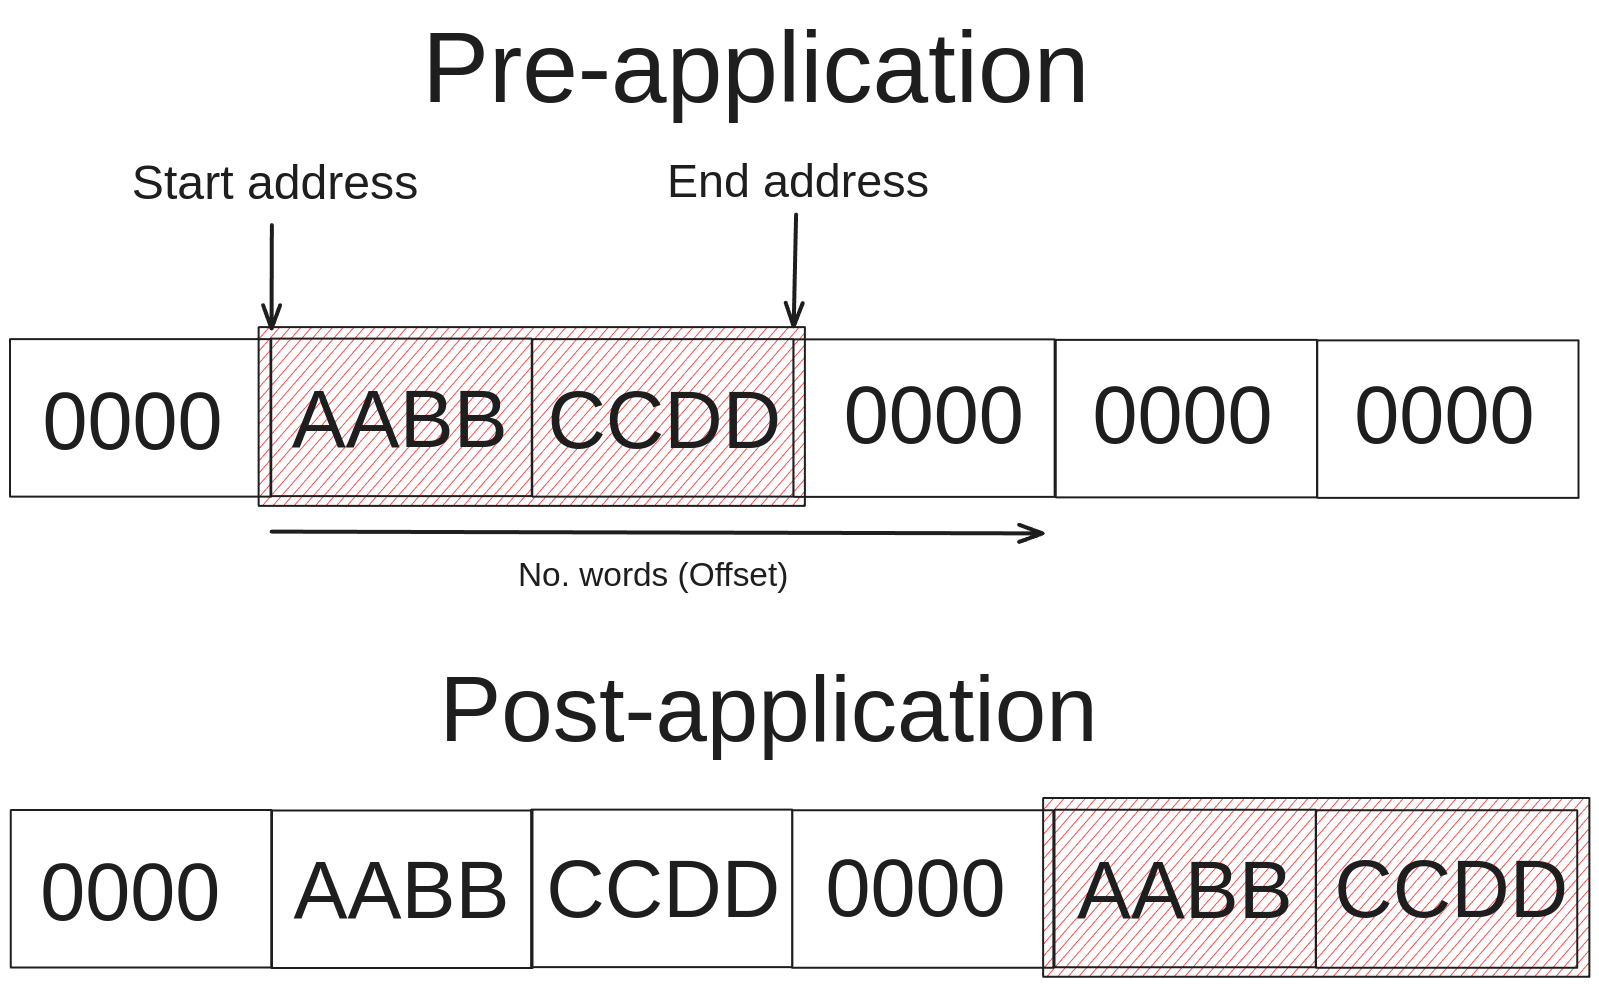
\includegraphics[width=\figurewidth]{img/shift_example.png}}
        }
        \caption{Visualisation of the shift operation.}
        \label{fig:shift_example}
    \end{shaded}
\end{figure}
After the \textbf{Shift} operation, additional instructions can safely be added to the newly made space with the \textbf{Write} operation. Note that the original range is left untouched by the \textbf{Shift} operation. The assumption is that the region will be used for new code and thus, will be overwritten imminently by another operation.

This is a more efficient way of describing the update as opposed to individual word-level changes, as there is no need to state already existing data. As one might expect, shifting a large portion of the binary image can be costly in terms of time, and the more code that is located posterior to the shifted region, the more costly the operation becomes. Methods to mitigate this cost are discussed in section \ref{sec:memory_layout}.

\textbf{\textit{Format.}} 
The \textit{diff} file is a text file that describes the changes to be made to the binary image. In this research, two main types of operations are considered: \textbf{Write} and \textbf{Shift}. The \textbf{Write} operation describes a change to a specific address, or range of addresses in the binary image, while the \textbf{Shift} operation describes a change that causes a portion of the binary image to be shifted. The format of the \textit{diff} file differs between operations, and below are some examples of the format.

\textbf{\textit{Write}:}
\begin{equation*}
    \overbrace{\textbf{W}}^{Operation}
    \overbrace{\textbf{1000A2}}^{Start\;address}    :
    \overbrace{\textbf{0004w}}^{No.\;Words}
    \overbrace{\textbf{FFFFFFFFFFFFFFFF}}^{Data}
\end{equation*}

\textbf{\textit{Shift}:}
\begin{equation*}
    \overbrace{\textbf{S}}^{Operation}
    \overbrace{\textbf{1000A2}}^{Start\;address}    \text{-}
    \overbrace{\textbf{1000B2}}^{End\;Address}      :
    \overbrace{\textbf{0004w}}^{No.\;Words}
\end{equation*}

\noindent The characters \textit{:}, \textit{-}, and, \textit{w} are used as separators, and all numeric fields are hexadecimal.

As the operations work fundamentally differently, the semantics of the fields of the \textit{diff} file depend on the operation. Specifically, in a \textbf{Write} operation, the \textbf{No. words} describes the length of the data field, while for a \textbf{Shift} operation, it describes the offset to shift by.

A detail that might seem inefficient is the use of a fixed size \textit{No. Words} argument with leading zeroes. However, during testing it was found that the overhead of these additional characters was less than the overhead of a variably sized field. The size of 4 hexadecimal digits, or 2 bytes, was chosen as it is the word size of the MSP430, and likely would be more than sufficient for the operations required in the DSU process. 

\section{The update procedure}\label{sec:updateprocedure}
With the main requirements of the implementation defined, the next step is to design an update procedure that meets the these requirements. The update procedure is the part of the process that is responsible for applying the patch file to the application. This is where the majority of the research conducted was focused. Firstly, for robustness and to simplify the implementation and testing, the update procedure was split into two phases: \textbf{Decode}, and \textbf{Apply}. This separation allows for the \textit{diff} file to be decoded and verified before the actual update is applied, an important property since the update procedure must be able to handle errors in the patch file, such as corruption or tampering. It also benefits debugging and profiling of the procedure, as the two phases can be tested separately. The following sections will describe these phases in further detail. 

\textbf{Decode.}
The Decode phase is responsible for reading the patch file and translating it into a format that can be used to apply the update. The patch file is read in one pass from the FRAM and decoded into a data structure that represents the changes to be made, which can be seen in listing \ref{lst:diff_struct}. 
\begin{framed}
    \begin{lstlisting}[
        caption={The data structure used to represent the changes in the patch file.},
        label={lst:diff_struct}
        ]
        typedef struct  
        {
            char      opcode;
            uint16_t  no_words;
            uint16_t* addr1;
            uint16_t* addr2;
            } diff_entry_t;
    \end{lstlisting}
\end{framed}
This data structure is then used in the Apply phase to apply the changes. The Decode phase is also responsible for verifying the integrity of the patch file, which in this research is of limited functionality, simply verifying that the patch file is in the correct format. To keep the implementation predictable in terms of memory usage, memory for the patch file, decoded patch instructions, and data is allocated at compile time in the FRAM of the device.

\textbf{Apply.}
The Apply phase is responsible for applying the changes to the binary image. The changes are applied in the order they are read from the patch file, and simply writes the new data to the specified addresses. This introduces the requirement that the patch file is ordered correctly, but this can be verified off the device. 

The Apply phase is a simple loop that iterates over the changes in the patch file and applies them to the specified addresses. An issue with the implementation is the lack of atomicity in the apply phase. If the update is interrupted, or fails for any reason, the system will be left in an inconsistent state. To counteract this, a rollback mechanism could be implemented using the same \textit{diff} file, but this is left to future work.

\section{Memory layout}\label{sec:memory_layout}
The MSP430FR5994 uses a unified memory model where FRAM, SRAM and registers can be accessed in the same memory space. The memory layout of the MSP430FR5994 can be seen in figure \ref{fig:memory_layout}.
\begin{figure}[!ht]
    \begin{shaded}
    \centering
    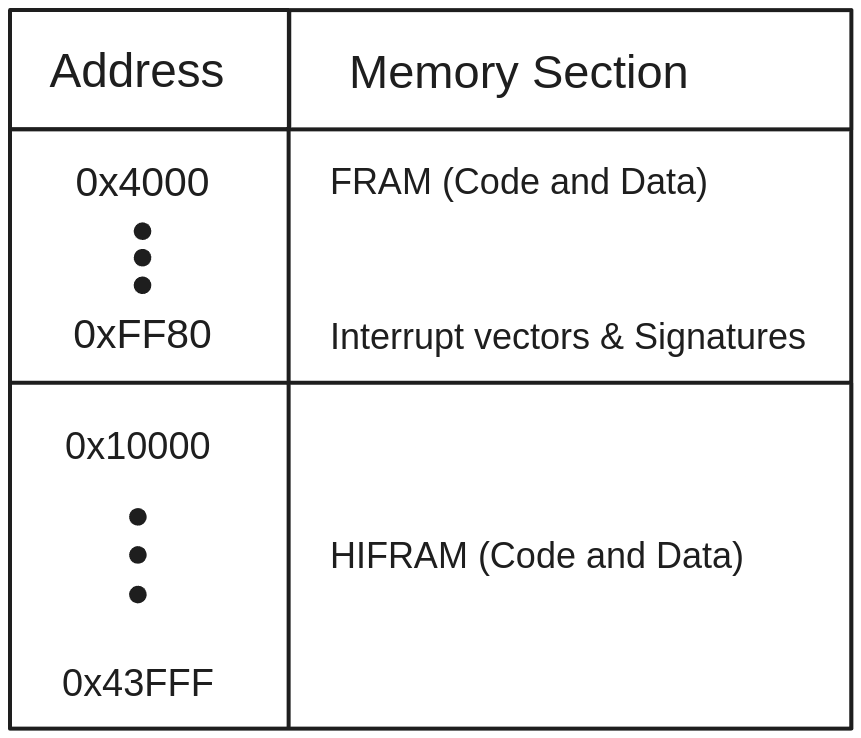
\includegraphics[width=\figurewidth]{img/mem_layout.png}
    \caption{Memory layout of the MSP430FR5994 microcontroller \cite{fr5994DataSheet}.}
    \label{fig:memory_layout}
\end{shaded}
\end{figure}

The figure has been simplified to highlight the important parts of discussion for this research. Essentially, all memory from address 0x4000 and up is the main memory used in any application running on the device. This is where the binary image of the program is stored, and where the update process will take place. The memory space is automatically divided into two sections by the compiler and linker, FRAM (0x4000-0xFFFF) and HIFRAM (0x10000 - 0x43FFF). This is due to the fact that the 16-bit architecture of the microprocessor doesn't natively allow addressing beyond 16-bit memory addresses. Accessing the HIFRAM section is only possible with an extension of the instruction set, using less efficient, emulated instructions. How these sections are used is up to the developer and can be configured in the linker script. 

To facilitate an efficient update process, the program should be structured in such a way that the added or removed code affects the rest of the program as little as possible. For example, moving a function in memory requires that all calls to said function are updated, which can be a time-consuming process. Additionally, adding new code within existing functions requires shifting everything directly below it, i.e. at higher addresses. Fortunately, the 2-section structure allows code within the FRAM section to be shifted without affecting the HIFRAM section, as there likely will be unused space between the two sections. However, in this research, the memory layout opted for is to have the DSU functionality in the FRAM section, with all other application code in the HIFRAM section. Using the open source \textit{gcc} compiler, the DSU functions are annotated with the \verb|lower| attribute, which forces the compiler to place the functions in the FRAM section. The program is then compiled with the \verb|-mlarge| and \verb|-mcode-region=upper| options, to place the rest of the program in the HIFRAM section. This way, the DSU code itself is never affected by the update process, which would almost certainly cause the update to fail. 

The drawback of this approach is that the application code is not as fast to access as it would be if it was stored in the FRAM section. This is a trade-off that was deemed necessary due to the decrease in complexity of any update performed.  
